%---------------------------------------------------
% کلاس سند: article برای اسناد متنی، با اندازه کاغذ A4 و فونت پایه 16
\documentclass[a4paper,16pt]{article}

% بسته‌های ریاضی برای معادلات و نمادهای پیشرفته
\usepackage{amsmath, amssymb, amstext}

% بسته رنگ برای استفاده از رنگ در متن یا محیط‌ها
\usepackage{xcolor}

% بسته گرافیک برای درج تصاویر
\usepackage{graphicx}

% تنظیمات حاشیه صفحه
\usepackage{geometry}

% بسته لینک‌دهی (هایپرلینک‌ها)
\usepackage{hyperref}

% بسته صفحه‌آرایی برای تنظیم هدر و فوتر
\usepackage{fancyhdr}


% بسته xepersian برای پشتیبانی از زبان فارسی با XeLaTeX
\usepackage{xepersian}

% تعیین فونت فارسی (فایل فونت باید موجود باشد یا در سیستم نصب باشد)
\settextfont{B Nazanin}

% تنظیم اندازه حاشیه‌ها از هر طرف برابر با 1 اینچ
\geometry{margin=1in}

% تنظیم سبک fancy برای سربرگ و پاورقی
\pagestyle{fancy}

% سمت چپ هدر: مشخص‌کننده سری تمرین و نام درس
\lhead{تمرین سری پنجم درس فیزیک\lr{II }}

% وسط هدر: نام دانشکده
\chead{دانشکده فیزیک دانشگاه صنعتی خواجه نصیرالدین طوسی}

% سمت راست هدر: تاریخ روز به‌صورت خودکار
\rhead{\today}

% پایین صفحه: شماره صفحه
\cfoot{\thepage}

% شروع سند
\begin{document}
	
	% صفحه عنوان (بدون هدر و فوتر)
	\thispagestyle{empty}
	\begin{center}
		% لوگوی دانشگاه (باید فایل تصویر در مسیر پروژه باشد)
		
		
\includegraphics[width=0.5\textwidth]{../../../images/image-E_5/image-1.png} \\[10pt] 
		% عنوان سند
		\textbf{\LARGE عنوان:تمرین سری‌پنج}\\[20pt]
		
		% نیم‌سال تحصیلی
		\textbf{\LARGE نیم‌سال تحصیلی:4032 }\\[10pt]
		
		% نام مدرس درس
		\textbf{\Large مدرس: ‫دكتر‬ ‫رضا‬ ‫افضل‬ ‫زاده‬}\\[10pt]
		
		% مبحث تمرین 
		\textbf{\Large ‫مبحث ‬‫تمرين‪:‬‬ ‫پايان‬ ‫ترم‬ }\\[10pt]
		
		% مهلت تحویل تمرین
		\textbf{\Large مهلت تحویل:22خرداد }
	\end{center}
	
	% صفحه جدید برای ادامه سند
	\newpage
	
	% ایجاد فهرست مطالب به‌صورت خودکار (براساس \section و \subsection و ...)
	\tableofcontents
	\newpage
	
	
	\section{سوال اول}
سيمی مطابق شكل حامل جريان ثابت \( I=125~\text{\lr{A}} \) است؛ ميدان مغناطيسی ناشی از يك بخش \( \ell=1~\text{\lr{cm}} \) از اين سيم را در نقطه‌ای به فاصله \( r=1.2~\text{\lr{m}} \) در حالات (الف) نقطه \(P_1\) و (ب) نقطه \(P_2\) بيابيد.

	\begin{center}
		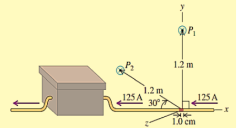
\includegraphics[width=0.5\textwidth]{../../../images/image-E_5/image-2.png} \\[10pt] 
	\end{center}
	
	\section{سوال دوم}
سيم راست و نازكی مطابق شكل در راستای محور \(x\) قرار دارد و جريان پايا \(I\) از آن می‌گذرد؛ ميدان مغناطيسی را در نقطه \(P\) به فاصله \(a\) از سيم به دست آوريد.

	
	\section{سوال سوم}
همان‌طور كه در شكل زير نشان داده شده است، يك حلقه مربعی از سيم با اضلاع
\( 2.0~\text{\lr{cm}} \)
داريم. ميدان مغناطيسی به سمت بيرون صفحه اعمال شده است كه مقدار آن به صورت
\[
B = 4.0\,t^{2} y
\]
داده می‌شود؛ كه در آن \(B\) بر حسب \(\text{\lr{T}}\)،
\(t\) بر حسب \(\text{\lr{s}}\) و
\(y\) بر حسب \(\text{\lr{m}}\) است. در زمان
\[
t = 2.5~\text{\lr{s}}
\]
\begin{enumerate}
	\item[(الف)] مقدار نيروی محركه الكتريكی القاشده را بيابيد.
	\item[(ب)] جهت نيروی محركه الكتريكی القاشده را تعيين كنيد.
\end{enumerate}
\begin{center}
	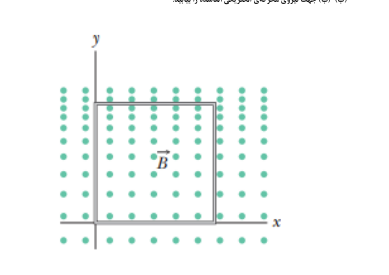
\includegraphics[width=0.5\textwidth]{../../../images/image-E_5/image-3.png} \\[10pt] 
\end{center}
	\section{سوال چهارم}
	يك سولنوئيد بلند با قطر \( d=12.0~\text{\lr{cm}} \) ميدانی يكنواخت با مقدار \( B=30.0~\text{\lr{mT}} \) ايجاد می‌كند كه با نرخ \( \frac{dB}{dt}=6.50~\text{\lr{mT/s}} \) كاهش می‌يابد؛ مقدار ميدان الكتريكی القاشده را در فاصله‌های (الف) \( r=2.20~\text{\lr{cm}} \) و (ب) \( r=8.20~\text{\lr{cm}} \) از محور سولنوئيد بيابيد.
	
	\newpage
	\section{سوال پنجم}
	
	در مدار شكل زير، جريان عبوری از مدار را محاسبه كنيد و اختلاف پتانسيل بين دو نقطه \(a\) و \(b\) را بيابيد. مقادير المان‌ها به صورت زير داده شده‌اند:
	\[
	R_1 = 3~\Omega , \qquad R_2 = 3~\Omega
	\]
	\[
	r_1 = r_2 = r_3 = 1~\Omega
	\]
	\[
	E_1 = 8~\text{\lr{V}}, \qquad E_2 = 12~\text{\lr{V}}, \qquad E_3 = 6~\text{\lr{V}}
	\]	\begin{center}
		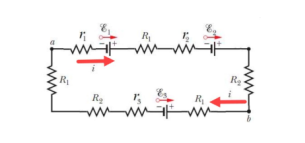
\includegraphics[width=0.5\textwidth]{../../../images/image-E_5/image-4.png} \\[10pt] 
	\end{center}
	\section{سوال ششم}
	دو خازنِ نشان‌داده‌شده در شكل ابتدا تا ولتاژ \(45~\text{\lr{V}}\) شارژ شده‌اند؛ (الف) چه مدت پس از بستن كليد، پتانسيل خازن‌ها به \(10~\text{\lr{V}}\) كاهش می‌يابد و (ب) مقدار جريان در اين زمان چقدر است؟
	\begin{center}
		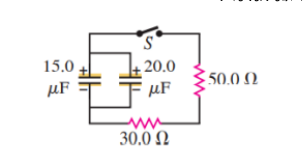
\includegraphics[width=0.5\textwidth]{../../../images/image-E_5/image-5.png} \\[10pt] 
	\end{center}
	
	\section{سوال هفتم}

در مدار شكل زير، جريان عبوری از هر شاخه را محاسبه كنيد. مقادير المان‌های مدار به صورت زير داده شده‌اند:
\[
R_1 = 2~\Omega , \qquad R_2 = 3~\Omega , \qquad R_3 = 4~\Omega
\]
\[
R_4 = 3~\Omega , \qquad R_5 = 5~\Omega , \qquad R_6 = 4~\Omega
\]
\[
r_1 = r_2 = r_3 = 1~\Omega
\]
\[
E_1 = 8~\text{\lr{V}}, \qquad E_2 = 12~\text{\lr{V}}, \qquad E_3 = 6~\text{\lr{V}}
\]
\begin{center}
	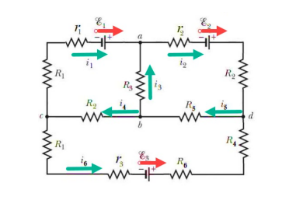
\includegraphics[width=0.5\textwidth]{../../../images/image-E_5/image-6.png} \\[10pt] 
\end{center}

	
	\textbf{موفق باشید.}
\end{document}
